\section{Approaches}
\label{sec:approach}

In the Blue Gene Q supercomputers, data transfers are routed along using default routing algorithm. The default routing algorithm is proved to be well-balanced in many communication patterns \cite{Chen:BGQ}. However, for certain communication patterns, it results in poor performance due to unbalanced networking load on physical links. In this section, we present four approaches aiming for balancing load on physical links. We also give a brief description of a framework called OPTIQ, a realizationf of our approaches.

\subsection{Path searching approaches}
Four approaches that we present in this section include two heuristic algorithms, one multiple paths data movement taking advantages of existing shortest paths algorithms and one model-based approach. All paths searching algorihtms here are centric algorithms i.e. run at every node in exact order. Hence, every node has the same results. The approaches need some information in advance such as size, topology, torus of the partition, coordinates of all nodes in the partition. The information is collected once at the begining. The algorithms also need to have tuples of data movement requests: source, destination and amount of data to be transferred from the source to the destination.

\subsubsection{Heuristic 1}
In this approach, we search for paths between each pair of source and destination. From a source, we explore from all the destination in all possible directions. Whenever we reach a destination, we mark the destination as found to no longer search for it on other explorering paths from the same source. In this algorithm, we do not limit exploring paths by any constraints. The algorithm is described in \textbf{Algorithm \ref{alg:h1}}.

\begin{algorithm}[!htp]
\textbf{Input:} Set of pairs of source-destination (\textit{s$_i$, d$_i$}). Number of nodes \textit{n}. Graph of nodes. \\
\textbf{Output:} Set of paths: one path for a pair of source-destination \\
\\
Structures:
\begin{algorithmic}
\State struct arc \{int u, int v\};
\State struct path \{set of arcs\};
\end{algorithmic}
Init:
    \begin{algorithmic}
	\State queue$<$struct path$>$ \textit{exploring\_paths} = $\varnothing$;
	\State queue$<$struct path$>$ \textit{complete\_paths} = $\varnothing$;
	\State bool \textit{visisted}[\textit{n}][\textit{n}];
	\For {0 $<=$ {\it i}, \textit{j} $<$ \textit{n}} 
	    \State \textit{visited}[{\it i}][{\it j}] = false;
	\EndFor
    \end{algorithmic}
Main:

\begin{algorithmic}
    \Function {Heuristic\_search\_I}{}

    \While {exist a source \textit{s$_i$} with unvisted neighbor \textit{u}}
	\State check\_and\_add\_new\_path({\it s}$_i$, \textit{u}, null);
	\State Pick next \textit{s$_i$} in the sources
    \EndWhile

    \While {(\textit{exploring\_path} != $\varnothing$)}
	\State path \textit{p} = \textit{exploring\_paths}.pop();
	\State {\it u} = last vertex in the path {\it p};
	\For {each neighbor \textit{v} of \textit{u}}
	    \State check\_and\_add\_new\_path({\it u}, \textit{v}, {\it p});
	\EndFor
    \EndWhile

    \EndFunction
\\
    \Function{check\_and\_add\_new\_path}{int \textit{u}, int \textit{v}, path {\it op}}
	\If {(!{\it visited}[{\it u}][{\it v}])}
	    \State create a path \textit{np} = {\it op}
	    \State add arc $<$\textit{u}, \textit{v}$>$ to \textit{np}
	    \State enqueue \textit{np} to \textit{exploring\_paths}
	    \If {{\it v} is one of the destinations of \textit{s$_i$} of \textit{np}}
	        \State enqueue \textit{np} to \textit{complete\_paths}
            \EndIf
	    \State {\it visited}[\textit{u}][\textit{v}] = true;
	\EndIf
    \EndFunction
\end{algorithmic}

\caption{Heuristic Alg 1: Exploring all paths without constraints}
\label{alg:h1}

\end{algorithm}

The \textbf{Algorithm \ref{alg:h1}} can be divided into 2 parts. In the first part, which is in the first \textbf{while} loop of the function Heuristic\_search\_I, we start at every source and add 1-hop paths to \textit{exploring\_paths} queue. Those paths are the paths from sources to their neighbors. We need a \textit{break} statement after each adding to make sure that every source can a path before they can all start again. This is to help ...

In the second part, which is the second \textbf{while} loop of the function Heuristic\_search\_I, we pop an exploring path \textit{p}from the \textit{exploring\_paths}. From the last added vertex \textit{u} of \textit{p}, we exploring all edges from it to it neighbors and add new path \textit{np} = \textit{p} + newly explored edge. If any of its neighbors is final destination of source \textit{s$_i$}, we then add \textit{np} into \textit{complete\_paths}. We continue the work until all the paths are explored.

Time complexity: The graph has V vertices and E edges. We have K pairs of (source, destinatinon), each source has at most D neighborhoods, then the time complexity of the \textbf{Algorithm \ref{alg:h1}} is $O$(K * (|V| + |E|)). The time complexity is breakdown as following:
\begin{itemize}
\item First part: we have K pairs hence K sources, for each source we discover its D neighbors, thus time will be $O$(K*D).
\item Second part: For this part, we get a path out of \textit{exploring\_paths}, create new paths by exploring its neighbors that are not visited by its source and add the new paths back to \textit{exploring\_paths}. For each sources, every vertex and every edge can be visited in the worst case, the time complexity would be $O$(|V| + |E|) minus to the vertices and edges visited by the first part. As we have K sources, the time complexity is $O$(K * (|V| + |E|)).
\end{itemize}

\subsubsection{Heuristic 2}
In the Algorithm \ref{alg:h1}, we explore all paths without concerning the number of hops that a path would take or maximum number of paths using a physical link. This leads to a long path or many paths sharing a physical link. A longer path results in more intermediate nodes, hence higher total transfer time. Higher maximum number of paths sharing a link leads to less bandwidth for each path. Both of them can lead to degraded performance.

This algorithm is an extension from Heuristic 1, in which we limit the exploring paths by both the number of hops and minimizing the maximum load. We do so by maintaining a min heap of paths. We use the heap to contain all the exploring paths instead of using a queue to manage the exploring paths as in Heuristic 1. This leads to increasing algorithm's time complexity in heap extracting (as taking data from a queue is O(1), from a min heap is O(log(n)) with n entries in the heap), but increasing the quality of explored paths. In this approach, we have finer results as we explore from least congested paths. The comparison function of the heap is based on both the number of hops and maximum load on each path. 

As most of the work in Heuristic 2 is similar to Heuristic 1, we do not repeat them, but only describe the differences between the two. The differences include:
\begin{itemize}
\item Use min heap of paths instead of queue of paths.
\item Need to heapify everytime we insert/delete from the min queue.
\end{itemize}

In the following, we describe the comparison function, which the core of the min heap for heapification. We also describe how to calculate the max load from the current load when adding a new path. We compare 2 paths based on its current max load and hop length. Among the two, max load has higher priority as max load affects the performance more.

\begin{algorithm}[!htp]

Heap element comparison:
    \begin{algorithmic}
	\Function{heap\_compare} {path p1, path p2, int maxload, int maxhops}
	    \If {both paths has max load greater than maxload} 
		\State choose the one with smaller number of hops.
	    \EndIf
	    \If {One path has max load greater but one path has max load smaller than maxload}
		\State Choose the one with smaller load.
	    \EndIf
        \EndFunction
    \end{algorithmic}

\caption{Heuristic Alg 2: Exploring all paths with hops length and max load constraints}
\label{alg:h2}
\end{algorithm}

\subsubsection{Heuristic 3}

\begin{algorithm}[!htp]
\textbf{Input:} Set of pairs of source-destination (\textit{s$_i$, d$_i$}). Number of nodes \textit{n}. Graph of nodes. Number of shortest path \textit{k}\\
\textbf{Output:} Set of paths: \textit{k} paths for a pair of source-destination\\
Init:
    \begin{algorithmic}
        \State queue$<$struct path$>$ \textit{complete\_paths};
    \end{algorithmic}
Main:
\begin{algorithmic}
    \Function {Heuristic\_search\_II}{}
	\For {each pair of source-dest (\textit{s$_i$}, \textit{s$_i$})}
	    \While{less than k paths discovered || still have paths to discover}
		\State Use Yen's algorithm to search for the shortest path \textit{p}.
		\State Check if adding \textit{p} make the current load over max load.
		\State If not, add \textit{p} into \textit{complete\_paths}
	    \EndWhile
	\EndFor
    \EndFunction
\end{algorithmic}

\caption{Heuristic Alg 3: k shortest paths}
\label{alg:h3}

\end{algorithm}

In the \textbf{Algorithm \ref{alg:h3}}, we use Yen's algorithm to search for k shortest paths between \textit{s$_i$, d$_i$}.

\begin{comment}

\subsubsection{Job-based AMPL model}
In this section we present a formal model written in A Modeling Language for Mathematical Programming (AMPL). The model captures demands of data movement between a set of sources and a set of destinations. The model also capture the graph of physical links of a partition given for the application. The model is presented in Model 1.

We presented the model in AMPL to solve the problem.

\begin{verbatim}
set Nodes;
set Arcs within Nodes cross Nodes;
set Jobs;

param Delay {Arcs} default 0;
param Capacity {Arcs} >= 0 default Infinity;
param Source {Jobs};
param Destination {Jobs} default 0;
param Demand {Jobs} default 0;

var Flow {Jobs, Arcs} >= 0;
var Z >= 0;

var total_flow{(i,j) in Arcs} = 
sum {job in Jobs} Flow[job,i,j];

maximize obj: Z;

subject to

zero_flow {job in Jobs, i in Nodes}:
sum{(i,j) in Arcs} Flow[job,i,j] - 
sum{(j,i) in Arcs} Flow[job,j,i] = 
if (i == Source[job])  then Demand[job]*Z 
else if (i == Destination[job]) then -Demand[job]*Z 
else 0;

capacity {(i,j) in Arcs}:
total_flow[i,j] <= Capacity[i,j];
\end{verbatim}

Model explanation:
\begin{itemize}
\item sets: we have 3 sets: \textit{Nodes}, \textit{Arcs} and \textit{Jobs}. \textit{JobID}: is the set of transfers from sources to destinations. Each job is represented by a tuple (id, source, destination, demand (total data size to transfer)).
\item params: {\it Delay}: delay on each arc; {\it Capacity}: capacity of each arc; {\it Source}: set of sources; {\it Destination}: set of destinations; {\it Demand}: amount of data to be transferred in each job.
\item vars: \textit{Flow}: total flow of each job on each arc; \textit{Z}: is reversed of total time; \textit{total\_flow} total flow of all jobs going through an arc.
\item objective function: we want to minimize the time or maximize its reversed value i.e. maximize \textit{Z}.
\item constraints(subject to): \textit{zero\_flow}: total flow through a source is total going out of that source, total flow going through a destination is total flow going in that destination, for other nodes that total is 0; \textit{capacity}: total flow on an arc is less than its capacity.
\end{itemize}

\end{comment}

\subsubsection{Path-based model}

\begingroup
\fontsize{9pt}{10pt}\selectfont

\begin{verbatim}

set Nodes;
set Arcs within Nodes cross Nodes;

set Jobs;
set Paths{Jobs};
set Path_Arcs{job in Jobs, p in Paths[job]} 
    within Arcs;

param Capacity{Arcs} >= 0 default Infinity;
param Demand {Jobs} default 0;

var Flow {job in Jobs, Paths[job]} >= 0;
var Z >= 0;

maximize obj: Z;

subject to

demand {job in Jobs}:
  sum {p in Paths[job]} Flow[job,p] = Demand[job]*Z;

capacity {(i,j) in Arcs}:
  sum {job in Jobs, p in Paths[job]: (i,j) in 
    Path_Arcs[job,p]} Flow[job,p] <= Capacity[i,j];

\end{verbatim}

\endgroup

Model explanation:
\begin{itemize}
\item sets: we have 5 sets: \textit{Nodes}, \textit{Arcs}, \textit{OD}, \textit{Paths} and \textit{Path\_Arcs}. \textit{JobID}: is the set of transfers from sources to destinations. Each job is represented by a tuple (id, source, destination, demand (total data size to transfer)).
\item params: {\it Capacity}: capacity of each arc; {\it Demand}: amount of data to be transferred in each job between a pair of orgin and destination.
\item vars: \textit{Flow}: total flow of each job on each arc; \textit{Z}: is reversed of total time; \textit{total\_flow} total flow of all jobs going through an arc.
\item objective function: we want to minimize the time or maximize its reversed value i.e. maximize \textit{Z}.
\item constraints(subject to): \textit{zero\_flow}: total flow through a source is total going out of that source, total flow going through a destination is total flow going in that destination, for other nodes that total is 0; \textit{capacity}: total flow on an arc is less than its capacity.
\end{itemize}

So far, we have presented different algorithms/approaches: here is when to use what:

\begin{table}[h]
\begin{center}
    \begin{tabular}{ | p{1.6cm} | l | p{3cm} |}
    \hline
    Approach & Time complexity & When to use \\ \hline
    Heuristic 1 & $O$(K * (|V| + |E|)) &  Used as first step for Heuristic 2\\ \hline
    Heuristic 2 & $O$(K * (|V| + |E|)) &  Very dense communication\\ \hline
    Heuristic 3 & $O$(K * (|V| + |E|)) & Sparse comminication \\ \hline
    Path-based model & $O$(K * (|V| + |E|)) & Medium dense where proportional throughtput can be gained \\
    \hline
    \end{tabular}

    \caption{Approaches: time complexity and usage}
    \label{tbl:experiment}

\end{center}
\end{table}

We realize algoirthms and other work in a framework named OPTIQ. The framework provides ways to improve data movement performance on the Blue Gene/Q supercomputer. Our framework does so by balancing loads on physical links on the Blue Gene/Q supercomputer.

\subsection{Framework}

Our framework has 3 main components: Path searching algorithms, Schedule and Transport and an extra component depicted in Figure \ref{fig:framework}.

\begin{figure}[!htb]
\vspace{-0.1in}
\centering
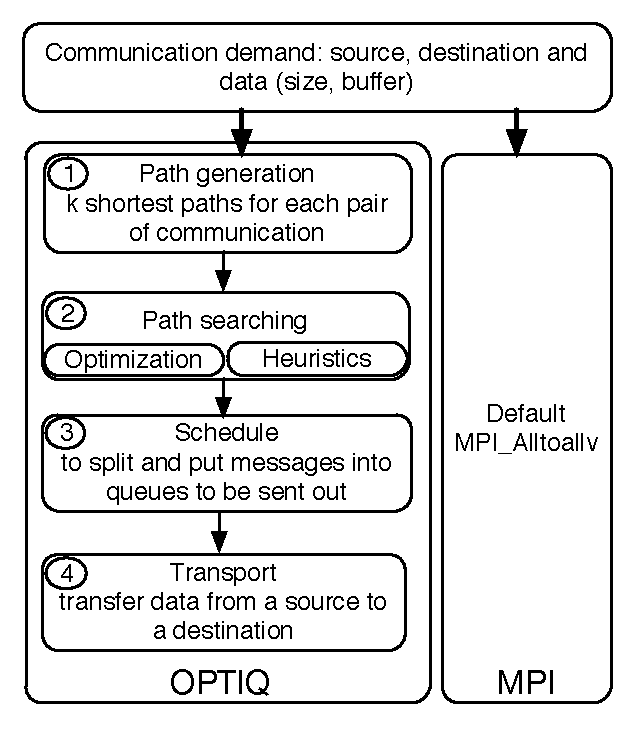
\includegraphics[scale=0.7]{figures/framework.pdf}
\vspace{-0.2in}
\caption{Three components of OPTIQ framework}
\vspace{-0.1in}
\label{fig:framework}
\end{figure}

The functionarity of each component is as following:
\begin{itemize}
\item Path searching: search for path to transfer data from a set of sources to a set of destination. Multiple or single paths can be found using a set of algorithm. User can decide what algorithm to be used or let the framework use a default algorithm.
\item Schedule: Split a buffer data that needed to tranfer into smaller messages and put those messages into a queue of transport layer to be transferred. It also handles incoming messages for itself and for forwardig them to its neighbors on a way to a message final destination.
As we route data in our own ways, we search for the paths, and we also need to schedule messages transfer. It includes sending local messages, forwarding messages form other sources, receiving data as the intermediate node or the destination node.

Order of messages into sending queue: 3 types of messages: local messages (needed to send), fowarding messages (needed to send), its receiving messages. first come first serve, local messages first. forwa

When there are multiple ranks per node, which one will be choosen to receive data at the next dest (forwarding). Single rank to do or many rank to do, currently every rank executes data transfer.

\item Transport: actually transfer an amount of data from one point to another point in the system.
\item Extra component: To get system specific information such as partition size, topology, coordinates, torus, and to compute neighbors of available nodes given to an application. Topology reading, coord, neighbors, torus, size, routing order, graph generated. Also set of benchmarks, tests.

the framework allow various options that allow to do: forwarding/local message sending order, algorithm selection, chunk size, transport implementations...
\end{itemize}
